\documentclass[a4paper,man,natbib]{apa6}
\usepackage{microtype}
\usepackage{mathtools} % needed
\usepackage{hyperref}
\usepackage{tabularx}
\usepackage{lingex}
\usepackage[modulo,displaymath,pagewise]{lineno}

\newcolumntype{Y}{>{\raggedright\arraybackslash}X}
\usepackage[normalem]{ulem}
\hypersetup{hidelinks=True}
\newcommand*{\smex}[1]{\textit{#1}} % 'small example'
\newcommand*{\spex}[1]{``{#1}''} % 'spoken example'
\newcommand*{\term}[1]{\emph{#1}} % introducing a new term
\newcommand*{\citegen}[1]{\citeauthor{#1}'s~(\citeyear{#1})}
\newcommand*{\SE}{\mathit{SE}} % fix funny "SE" spacing
\newcommand{\resultsLog}[3]{$\beta = #1$, $\textnormal{SE} = #2$, $p #3$}
\newcommand{\resultsLM}[3]{$\beta = #1$, $\textnormal{SE} = #2$, $t #3$}

\usepackage[obeyFinal,textsize=tiny,backgroundcolor=yellow!60,linecolor=black!60]{todonotes} % to get rid of all notes, pass
% `final' to the document class
\setlength{\marginparwidth}{2cm}
\let\oldtodo\todo
\renewcommand*{\todo}[1]{\oldtodo[fancyline]{#1}}

\title{Such gesture, very lie, wow}
\author{reorder(MC,JK,JL)}
\affiliation{Psychology, PPLS, University of Edinburgh}
\ifapamodeman{\note{\begin{flushleft}%
Josiah King\\
Philosophy, Psychology and Language Sciences\\
University of Edinburgh\\
7~George Square\\
Edinburgh EH8~9JZ, UK\\[1ex]
\url{J.P.J.King@sms.ed.ac.uk}
\end{flushleft}}}

\abstract{
Previous research suggests that, when questioning the veracity of an utterance, we perceive certain non-linguistic behaviours to indicate that a speaker is being deceptive.
Recently, work has highlighted how listeners' associations between speech disfluency and dishonesty happen at the earliest stages of reference comprehension, suggesting that the manner of spoken delivery influences pragmatic judgements concurrently with the processing of lexical information.
The studies presented here investigate the integration of visual information about a speaker into judgements of deception.
By studying the time course of judgements of a speaker's (dis)honesty when presented with different visual cues to deception, we ask whether listeners are relying upon a rule-of-thumb association between visual cues and deception, or whether the link between gestures and perceived deception requires a more complex inferential process.
Participants saw and heard a video of a potentially dishonest speaker describe treasure being hidden behind a named object, while also viewing both the named object and a distractor object. 
Their task was to click on the object behind which they believed the treasure to actually be hidden.
Eye- and mouse-movements were recorded. 
Experiment~1 investigates listeners' associations between visual cues and deception, using a variety of static and dynamic cues, with Experiment~2 clarifying the time-course of judgements of deception based on adaptor gestures. 
Results show that the visual modality can have a rapid and direct influence on pragmatic judgements, supporting the idea that communication is fundamentally multimodal.
Although the nonverbal delivery of an utterance is found to influence the early stages of reference comprehension, establishing deception-judgements based on visual cues appears to be more gradual than previous studies have suggested it is for spoken cues.
}


\begin{document}

\shorttitle{What do liars look like?}
\maketitle
\linenumbers
\noindent
In natural communication, speakers can convey information via multiple channels.
Along with spoken delivery, a speaker's gestures, postures and facial expressions all offer information which can have a bearing on the non-literal (or pragmatic) interpretation of a message, for instance conveying emotion \citep{Busso2004, Gregersen2005}.
One such pragmatic interpretation is the judgement of a statement's veracity.
Research suggests that there are many aspects of nonverbal delivery which we, as listeners, believe to be \term{cues-to-deception}. 
In an analysis of 33~studies, \citet{Zuckerman1981} found that nine out of the ten visual cues-to-deception that were investigated were believed to be indicative of deceit. 
In a further subset of 13~studies reporting relationships between cues and subsequent deception judgements (rather than explicit beliefs about cues), three (smiling, gaze, and postural shifts) of the four available visual cues were associated with perceived dishonesty.

Interestingly, listeners appear to make these associations independent of the reliability of cues as actual signals of deception: \citet{Zuckerman1981} found only two visual cues (shrugs and fidgetting) to be associated with actual deceit, and a more recent meta-analysis found little evidence of a relationship between lying and almost any form of movement \citep{DePaulo2003}.
Some studies have in fact found deception to be inversely related to the cues we think of as deceitful:
Lying has been linked with a \emph{decrease} in hand, arm, and leg movements \citep[e.g.][]{DePaulo1992, Ekman1989, Vrij1995}, as well as a reduction in illustrative gesturing \citep[e.g.][]{DePaulo2003, Cohen2010}.
Even speakers' post-hoc perceptions of their own gestures when lying have been found to be at odds with how they actually behave:
\citet{Vrij1996} found that after partaking in interviews in which they were in turn truthful and dishonest, participants believed that their movements increased when lying, even though a decrease actually occurred.
An alternative view suggested by \citet{Hartwig2011} is that listeners are not relying on the wrong cues when forming judgements of deception, it is simply that associations between behavioural cues and lying are weak \citep{Hartwig2011}.

Whether listeners intuitions about deceitful behaviour are misjudged or merely exaggerated, the associations they make between visual information and deception are unlikely to have been learnt.
This is reinforced by the fact that in everyday communication, there are few occurrences where listeners are given immediate feedback on the honesty of a given utterance.
Why do listeners associate certain behaviours with deceit, and how are they incorporated into the judgements listeners make about whether or not an utterance is true?
One suggestion is that listeners judgements might follow simple and straightforward rules-of-thumb, relying on heuristically associating certain cues with deception \citep{DePaulo1982}.
The heuristics may be predicated on lay beliefs about deception, or on introspection as a speaker rather than experience as a listener.
For instance, if people believe they themselves fidget more when they lie, they may be inclined to interpret fidgeting in others as cues to deception.
Following a rule-of-thumb like this would mean listeners' judgements about whether or not someone is lying can occur quickly and with little effort.

\citet{Loy2017} investigated the association between lying and speech disfluency, and found support for the idea that listeners rely on a rule-of-thumb-based approach when judging the veracity of an utterance based on the way in which it is spoken.
\citeauthor{Loy2017} used a visual world eye- and mousetracking paradigm in which participants were presented with images of two objects, and heard utterances describing the location of some treasure purportedly hidden behind one of the objects.
These utterances were presented as having been elicited in a previous experiment, in which the speaker was said to have been lying some of the time.
Crucially, \citet{Loy2017} manipulated the manner of spoken delivery, with half of the experimental items containing a speech disfluency.
Participants were tasked with clicking on the object they \textit{believed} to be concealing the treasure, choosing either the object named in the utterance (indicating a judgement of honesty), or a distractor (indicating dishonesty).
They were more likely to judge disfluent utterances as dishonest than fluent ones (as indicated by a greater probability of clicking on the distractor in a disfluent trial). 
Importantly, disfluency resulted in an early bias in both eye and mouse movements towards the not-referred-to object.
This suggests that speech disfluency is already incorporated into listeners' ideas concerning deceptive speech, and has an immediate effect on their interpretation of an utterance. 

It seems reasonable to assume that the early effects of speech disfluency reflect a rule-of-thumb association of disfluency with dishonesty.
In fact, any rule-of-thumb may be quite general:  Evidence suggests, for example, that some effects of speech interruptions on comprehension are not sensitive to differences between a spoken \spex{um} and an artificial tone \citep{Corley2011}.
Co-speech movements, however, are substantially more varied than speech interruptions, serving as both potential markers of metacognitive states and planning processes, and as an alternative modality in which a speaker can convey semantic information (such as via an illustrator).
Any rule-of-thumb linking visual information to deception would have to be refined enough to discriminate types and contents of co-speech movements, or risk potentially over-attributing any cue as a sign of deceit.
Furthermore, listeners associate static visual cues with deception \citep[e.g. eye-gaze,][]{Zuckerman1981a}, suggesting that judgements of dishonesty are not linked just to variations in movement, but to a wide array of visual cues. 

An alternative to the heuristic explanation suggests that non-linguistic information might influence listeners' judgements of deception via a form of on-the-fly speaker modelling: 
When presented with a possibly deceitful utterance, listeners might be inferring information about a speaker's metacognitive states, linking visual and spoken cues to deception via the perception of, e.g., nervousness, or cognitive effort. 
Such an account requires more complex inferential processing.
Participants would have to make links between specific visual cues and metacognition, which would in turn be linked to a judgement of veracity.

To date, the link between visual cues and perceived deceit has been studied only in terms of after-the-fact judgements, or assessing listeners' explicit beliefs about cue validity (see \citealt{Vrij1996a, Zuckerman1981a}).
In the two experiments presented here, we extend the `treasure game' paradigm from \citet{Loy2017} to include a video of a potentially deceptive speaker describing the location (behind one of two objects) of some hidden treasure on the screen (see \ref{fig:v1_layout}).
Crucially, we manipulate the presence or absence of potential visual cues to deception in the video.
Listeners attempt to guess, and click on, the true location of the treasure, which allows us to infer whether they believe the speaker to be lying or telling the truth.
If listeners associate given a visual cue with deception, they should be more likely to click on the object which has not been mentioned.
By measuring listeners' eye- and mouse-movements as the speaker's descriptions unfold, we can investigate their interpretations of what is being said over time.
To the extent that this bias occurs early during relevant trials, it is possible to infer that listeners are acting on a heuristic association between cue and falsehood.

\begin{figure}[Ht]
  \centering
	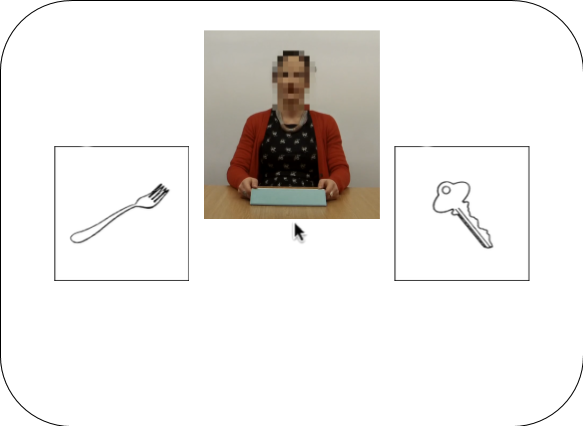
\includegraphics[width=\linewidth]{./img/e7_layout.png}
  \caption{Visual world with video stimulus}
  \label{fig:v1_layout}
\end{figure}

In Experiment~1, we focus on how trunk movements (postural shifts) influence judgements of utterance veracity, with filler trials presenting two further types of visual cue (adaptor gesturing, and different static postures).
The decision to focus on trunk movements was twofold: Firstly, previous research indicates that these movements are associated with perceived lying\citep{Vrij1996a}, and secondly, they offer practical advantages in integrating a video stimulus into the visual-world paradigm, as we require visual cues to be both salient enough for participants to notice them, but not to detract from fixations to objects at the onset of the critical noun.
Videos of trunk movements involve movement over a larger area of the video than hand or head movements, and appear believable when presented with little or no overlap with speech, providing a visual cue comparable to the utterance-initial disfluency in \citet{Loy2017}.

Interestingly, the results from Experiment~1 indicate that the filler items, specifically adaptor gestures, are more strongly associated with deception, and when presented alongside speech (rather than before, as for trunk movement) they do not detract from seeing this association emerge in the early stages of comprehension.
Because the videos presented in filler trials in Experiment~1 are not fully counterbalanced, and may be influenced by other design factors (see below), we conducted Experiment~2 to clarify the time course of deception judgements based on visual cues, looking excusively at adaptor gestures.


\section{Experiment~1}
Experiment~1 makes use of eye- and mouse-tracking to investigate whether visual cues affect listeners' judgements about the veracity of an utterance over time. 
The experiment was presented as a `lie detection game'.
Each trial included a video and audio recording of a potentially deceptive speaker describing the location of some hidden treasure on the screen.
Throughout a trial, two images, depicting potential treasure locations, remained visible. 
Participants were tasked with using the mouse to click on the object they believed to be concealing the treasure.
Critical trials presented videos of the speaker either producing a trunk movement immediately prior to utterance playback, or sitting motionless (no cue) for the equivalent amount of time.
Filler trials presented videos of the speaker producing no cue, sitting in a different posture, or producing an adaptor gesture. 
Our aim was to investigate whether and when particular cues would be associated with falsehood.
%% (add) Our results show that...


\subsection{Materials}
Visual stimuli consisted of the same 120 line drawings from \citet{Snodgrass1980} which were used in \citet{Loy2017}, sixty of which served as the object named as hiding the treasure and the other sixty as distractors.
Referents were randomly paired with distractors and presented across sixty trials (20 critical and 40 fillers). 
In each trial, the speaker named one object (referent) as that which concealed the treasure; the other object is hereafter named the distractor.
Each referent was associated with a recording of fluent speech specifying the image as the object that the treasure was hidden behind (``The treasure is behind the <referent>'').
Along with these images, each trial presented a video (with no audio) of a person who was purported to be the speaker of the utterances. 
So that videos could be counterbalanced across referents, and thus across utterances, the face of the person in the video was blurred. 
This meant that, when presented with a given utterance, it was believable that both audio and visual stimuli had been produced concurrently. 

Thirty-five videos were created.
Ten of these showed a speaker sitting motionless with her hands on either side of a tablet (upon which the referent, distractor, and treasure was purported to be displayed) which was resting on a table.
These ten videos were each seen in one critical trial, and were repeated in two filler trials.
Five videos of trunk movements were each presented in two critical trials each.
The remaining 20 videos (each presented in one filler trial) showed the speaker either producing an adaptor gestures such as finger-tapping or head-tilting (10 videos) or sitting motionless but in a different, non-neutral posture such as hand-on-chin or arms crossed (10 videos).
This meant that over the course of the experiment each participant saw 30 videos of the speaker producing no cue, and 30 videos of the speaker producing some type of cue (10 showing trunk movements; 10 showing adaptor gestures; 10 showing different postures).

To ensure that audio and video presented together appeared believable, each video was assigned a frame number corresponding to the point at which audio was to begin.
For videos showing a trunk movement, this was the frame at which the movement ended, meaning that participants were presented with no overlap between the movement and speech (Ranging from 23-56 frames with a median of 37). 
The frame numbers for trunk movements were matched in videos showing no cue, thus controlling for any sensitivity to the duration of video prior to speech (which could be interpreted as speech-initiation time, in turn a potential cue to deception). 
For videos showing an adaptor gesture, the frame at which audio began was individually determined based on what looked most believable to the researchers (Ranging from 21-53 frames with a median of 36.5), and so the amount of overlap between movement and speech varied.
These frame numbers were matched in the videos showing the speaker in different postures.

As with \citet{Loy2017}, 20 critical referents were counterbalanced across two lists. 
Each list contained 10 trials showing a trunk movement video and 10 trials showing a video showing no cue.
The remaining 40 referents were randomly paired with one of the remaining videos (10 showing adaptor gestures, 10 showing different postures, 20 showing no cue) for each participant, with no repetition of referents across videos.

\subsection{Procedure}
Stimuli were displayed on a 21~in.\@ CRT monitor with a resolution of 1024~$\times$~768, placed 850~mm from an Eyelink~1000 Tower-mounted eye-tracker which tracked eye movements at 500~Hz (right eye only). 
Audio was sampled at 44100~Hz and presented in stereo from speakers on either side of the monitor. 
Mouse coordinates were sampled at the frame rate of the videos (25~fps, or every 40~ms).
The experiment was presented using OpenSesame version~3.1 \citep{Mathot2012}.
Eye movements, mouse coordinates and object clicked (referent or distractor) were recorded for each trial.

Figure \ref{fig:v1_trial} presents a sample trial from the experiment. 
\begin{figure}[Ht]
  \centering
	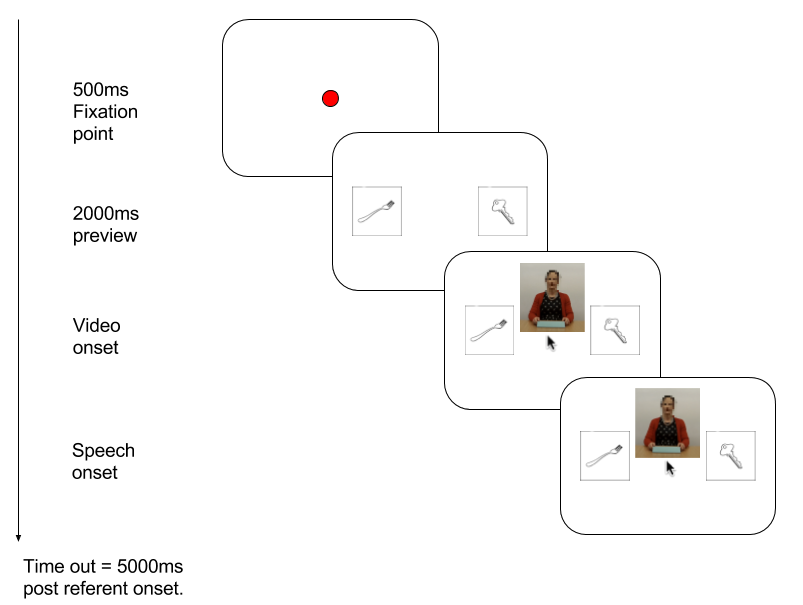
\includegraphics[width=\linewidth]{./img/e7_trial.png}
  \caption{Procedure of a given trial, Experiment~1}
  \label{fig:v1_trial}
\end{figure}
Between trials, participants underwent a manual drift correct to ensure accurate recordings from the eye-tracker.
After this the fixation dot turned red for 500ms to signify progression to the trial. 
This was replaced by the two images of the referent and distractor, measuring 150~$\times$~150 pixels, centered vertically and positioned such that the center of each object was 15\% from either edge of the display. 
The relative positions (Left vs.\@ Right) of referents and distractors was randomly chosen, with the constraint that for each participant saw the referent in an equal number of critical and filler trials on the left as on the right.
This display lasted for 2000~ms before the video was added and the cursor was centred and made visible.
The video, measuring 266~$\times$~284 pixels, was displayed with the bottom edge at the middle point vertically, and centered horizontally.
Playback of the utterance began at the assigned frame of the video.
The trial ended once the participant clicked on either object, or 5000~ms after the onset of the referent noun.

The instructions emphasised that the videos participants saw were recorded from a previous experiment, in which the speaker had to describe the location of some hidden treasure with the aim of misleading the listener into choosing the wrong location.
Participants were told that the speakers in the previous experiment would lie approximately half of the time. 
Participants were instructed to click on the object behind which \textit{they believed} the treasure to be hidden, with the overall aim of accumulating as much treasure as they could across the experiment.
Participants received no feedback after their object clicks, except on bonus trials, which are described in the next section.

The order of trials was randomly assigned on each run of the experiment.
Participants completed five practice trials (one of which was presented as a bonus round) prior to the main experiment. 
Two of these presented a video showing no cue, two displayed a video of the speaker in different postures, and one displayed a video of the speaker making a trunk movement.


\subsection{Bonus Rounds}
To maintain motivation throughout the study, participants were told that there were a number of ``hidden bonus rounds'' which offered more treasure than regular rounds.
25\% of filler trials (half presenting a video showing either adaptor gesturing or a different posture; half presenting a video showing no cue) were randomly designated as bonus rounds for each participant.
These trials were visually identical to regular trials, with the exception of a message informing participants that they had successfully located bonus treasure following their mouse click (regardless of the object chosen).
Participants were also told that the top scorers would be able to enter their names on a high-score table, which was shown at the beginning of the experiment. 

\subsection{Post-test Questionnaire}
Participants were asked to complete a short post-test questionnaire which asked whether participants had noticed anything odd about the visual or audio stimuli.
Any participant who indicated that they had noticed anything unusual was then questioned further, to decide whether they believed that the speech and gesture had been produced naturally and simultaneously.
All participants were subsequently debriefed, during which they were told that the audio and video were created separately and stitched together, and asked again verbally if they noticed anything unusual in that respect. 
Responses to the questionnaire and debrief were used as exclusion criteria for the analysis.

\section{Results}
Twenty-four native English speaking participants took part in the experiment for a planned sample size of twenty.
Participants were recruited from the University of Edinburgh community, and participated in return for a payment of \pounds{}4.
Data from four participants who indicated suspicion of the proposed origins of the audiovisual stimuli based on the post-test questionnaire and/or debrief were removed from all analyses.

\subsection{Analysis}
Analysis of critical trials was carried out in R version~3.4.4 \citep{Rbase2017}, using the lme4 package version~1.1-17 \citep{Bates2015}. 
Trials in which participants did not click on either the referent or distractor were excluded from all analyses (1 of 400 critical trials).

Object clicked (referent or distractor) was modeled using mixed effects logistic regression, with a fixed effect of type of visual cue (no cue, trunk movements, different postures, adaptor gestures), deviation coded, with random intercepts and slopes for cue type both by-participant and by-item
Reaction times (measured from referent onset) were log transformed and modelled with the same fixed and random effect structure using mixed effects linear regression.

Eye fixation data was averaged into 20~ms bins (of 10 samples) prior to analysis.
For each bin, we calculated the proportions of time spent fixating the referent or the distractor, resulting in a measure of the proportions of fixations on either object over time.
The position of the mouse was sampled every 40~ms.
Using the $X$ coordinates only, we calculated the number of screen pixels moved and the direction of movement (towards either referent or distractor).
We then calculated the cumulative distance travelled towards each object over time as a proportion of the cumulative distance travelled in both directions from referent onset up until that time bin.
Movements beyond the outer edge of either object were considered to be `overshooting' and were not included in calculations (0.8\% of samples).
Eye- and mouse- biases were calculated from the proportions of referent to distractor fixations, and were subsequently empirical logit transformed \citep{Barr2008}. 
In these measures, a value of zero indicates no bias towards either object, and positive and negative values indicate a bias towards the referent and distractor respectively.

As in previous studies using the treasure game paradigm \citep{King2018,Loy2017}, eye- and mouse- tracking analyses were conducted on a time-window beginning at referent onset and extending for 800~ms, just beyond the duration of the longest referent (776~ms).
Eye and mouse data was modelled over this time window using linear mixed effects models, with fixed effects of time from referent onset (seconds), type of cue, and their interaction.
Type of cue was dummy coded with no cue as the reference level.
Random intercepts and slopes for time and cue type were included both by-item and by-participant.
Following \citet{Baayen2008}, we considered effects in these models to be significant where $|t|>2$.

Filler trials (800) were analysed in the same way, with two differences. 
Firstly, in all models, by-item random effects for type of cue (Now comprising three levels: no cue, different postures, and adaptor gesturing) were removed as they were not counterbalanced across referents.
Secondly, eye- and mouse- tracking analyses was extended to the 1100~ms following onset of the referent. 
This decision was based on the fact that the longest referent in filler trials was 1062~ms. 
Filler trials resulting in no mouse click on either object (3) were excluded from these analyses.

\subsection{Object clicks} 
Across the experiment, participants clicked on the referent in 55\% of trials and the distractor in only 45\%.
Table \ref{table:v1_clicks} shows the percentage of clicks across all participants to either object following videos showing different types of cue.

Analysis of critical trials indicated that visual information about the speaker had marginal effect on participants decisions to click on either object, with videos showing no cue resulting in marginally more clicks towards the referent (\resultsLog{0.28}{0.16}{0.08}).
There was no effect of cues on the time taken by participants to click on an object.

Analysis of filler trials found that videos showing the speaker producing adaptor gestures (but not those showing the speaker in different postures) were associated with final judgements of deception, as participants were more likely to click on the distractor than the referent following these videos (\resultsLog{-0.44}{0.16}{0.006}).
The type of cue shown in the video not associated with any significant changes in the time taken by participants to click on an object.

\begin{table}
\caption{Breakdown of mouse clicks recorded on each object (referent or distractor) by type of visual cue for Experiment~1}
\label{table:v1_clicks}
\begin{tabularx}{\linewidth}{YYYYY}
\hline
& No-Cue & Trunk Movement & Different Posture & Adaptor Gesture \\
Clicks to Referent & 96 (48.0\%) & 381 (63.8\%) & 99 (49.7\%) & 83 (41.5\%)  \\ 
Clicks to Distractor & 104 (52.0\%) & 216 (36.2\%) & 100 (50.3\%) & 117 (58.5\%) \\
\hline
\end{tabularx}
\end{table}

\subsection{Eye movements}
Figure \ref{fig:v1_eye1} shows the time course of fixations to referents and distractors in critical trials for the 2000~ms from referent onset, split by the type of cue shown in the video (no cue or a trunk movement).

Analysis of critical trials conducted over the period from referent onset to 800~ms post-onset (duration of the longest referent) showed that when presented with a video showing no cue, participants showed a bias towards towards fixating on referent which increased over the course of the window, as indicated by a main effect of time (\resultsLM{2.23}{0.67}{=3.34}).
There were no main effects of type of cue, nor any interaction of cue type with time, indicating that whether the video showed the speaker either producing a trunk movement or sitting motionless did not influence participants tendency to fixate upon the referent.


Analysis of filler trials (conducted from referent onset to 1100~ms) showed the same tendency to fixate towards the referent over the distractor in trials presenting a video showing the speaker producing no cue (\resultsLM{1.05}{0.34}{3.13}).
Figure \ref{fig:v1_eye2} shows the time course of fixations to referents and distractors in filler trials for the 2000~ms from referent onset, split by the type of cue shown in the video (no cue, different postures, or adaptor gesturing).
Relative to videos showing no cue, when participants viewed videos which presented the speaker either in a different posture or producing an adaptor gesture, the increasing bias over time toward the referent was significantly reduced (\resultsLM{-0.97}{0.13}{=-7.23} and \resultsLM{-0.58}{0.13}{=-4.38} respectively).

\begin{figure}[Ht]
  \centering
	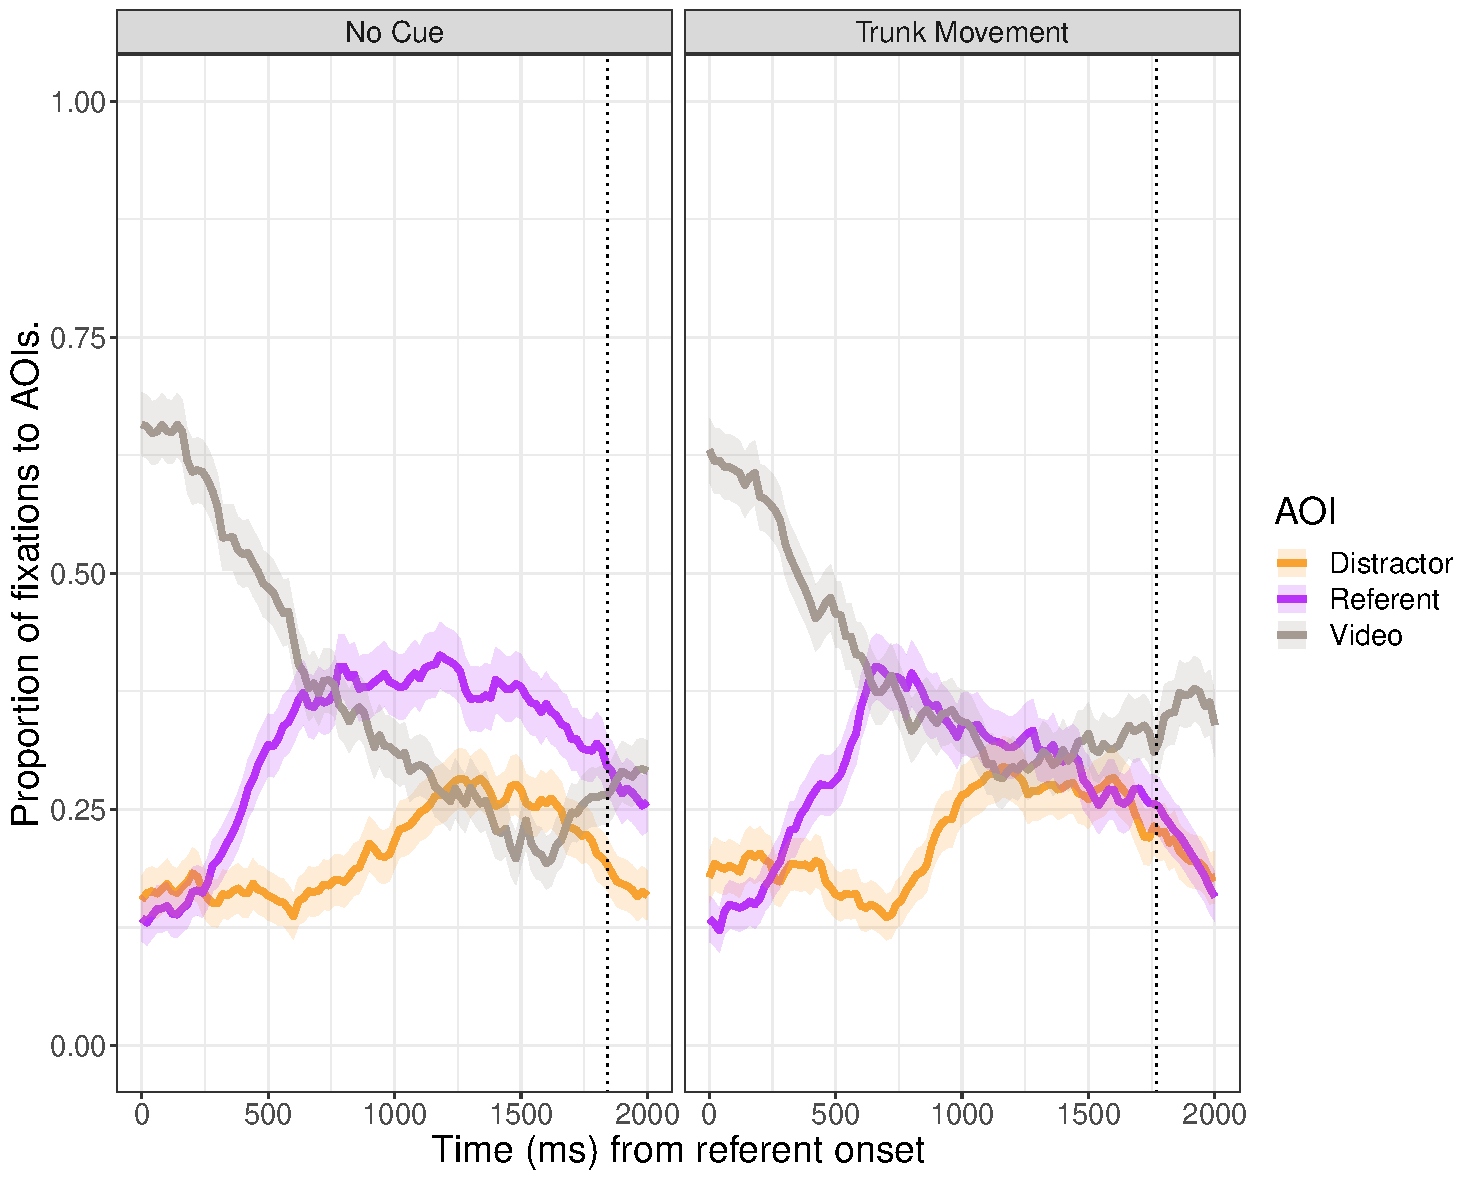
\includegraphics[width=\linewidth]{./img/e7_fixations_crit.pdf}
  \caption{Eye-tracking results for critical trials in Experiment~1: Proportion of fixations to each object (referent or distractor) and the video, from 0 to 2000 ms post-referent onset, calculated out of the total sum of fixations for each 20~ms time bin. Shaded areas represent $\pm$ 1 standard error of the mean.}
  \label{fig:v1_eye1}
\end{figure}

\begin{figure}[Ht]
  \centering
	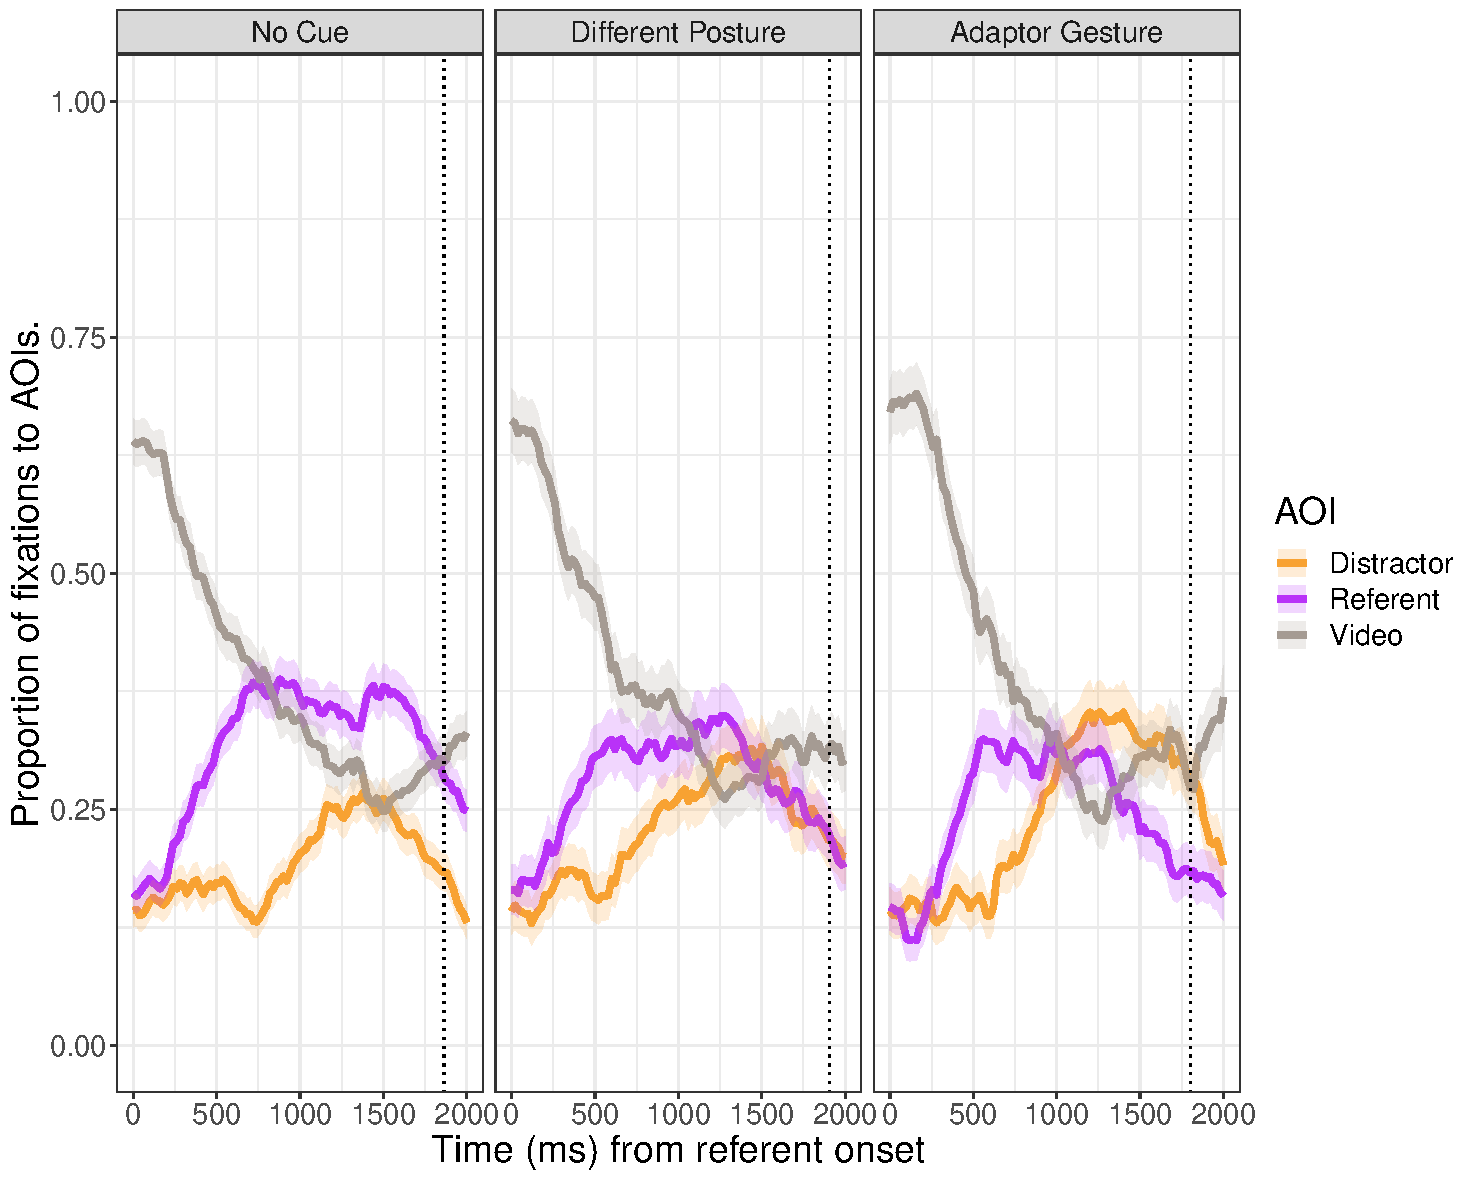
\includegraphics[width=\linewidth]{./img/e7_fixations_filler.pdf}
  \caption{Eye-tracking results for filler trials in Experiment~1: Proportion of fixations to each object (referent or distractor) and the video, from 0 to 2000 ms post-referent onset, calculated out of the total sum of fixations for each 20~ms time bin. Shaded areas represent $\pm$ 1 standard error of the mean.}
  \label{fig:v1_eye2}
\end{figure}


\subsection{Mouse movements}
Figure \ref{fig:v1_mouse1} shows the time course of the proportions of cumulative distance the mouse moved towards the referent and distractor in critical trials for 2000~ms from referent onset, split by each type of cue.


Analysis of critical trials on the 800~ms following referent onset patterned with the eye movements:
Participants showed an increasing bias over the course of this window to move towards the referent when the video showed the speaker presenting no cue (\resultsLM{0.77}{0.33}{2.36}), and this was not found to change for videos presenting the speaker producing a trunk movement.

Figure \ref{fig:v1_mouse2} shows the time course of the proportions of cumulative distance the mouse moved towards the referent and distractor in critical trials for 2000~ms from referent onset, split by each type of cue.
Analysis of mouse movements in filler trials also patterned with analysis of eye-movements for these trials:
Relative to videos showing no cue, the tendency to move towards the referent over the distractor (\resultsLM{1.08}{0.23}{4.62}) was significantly reduced for videos showing the speaker either in a different posture or producing an adaptor gesture (\resultsLM{-0.54}{0.12}{-4.52} and \resultsLM{-0.86}{0.12}{-7.19} respectively).

\begin{figure}[Ht]
  \centering
	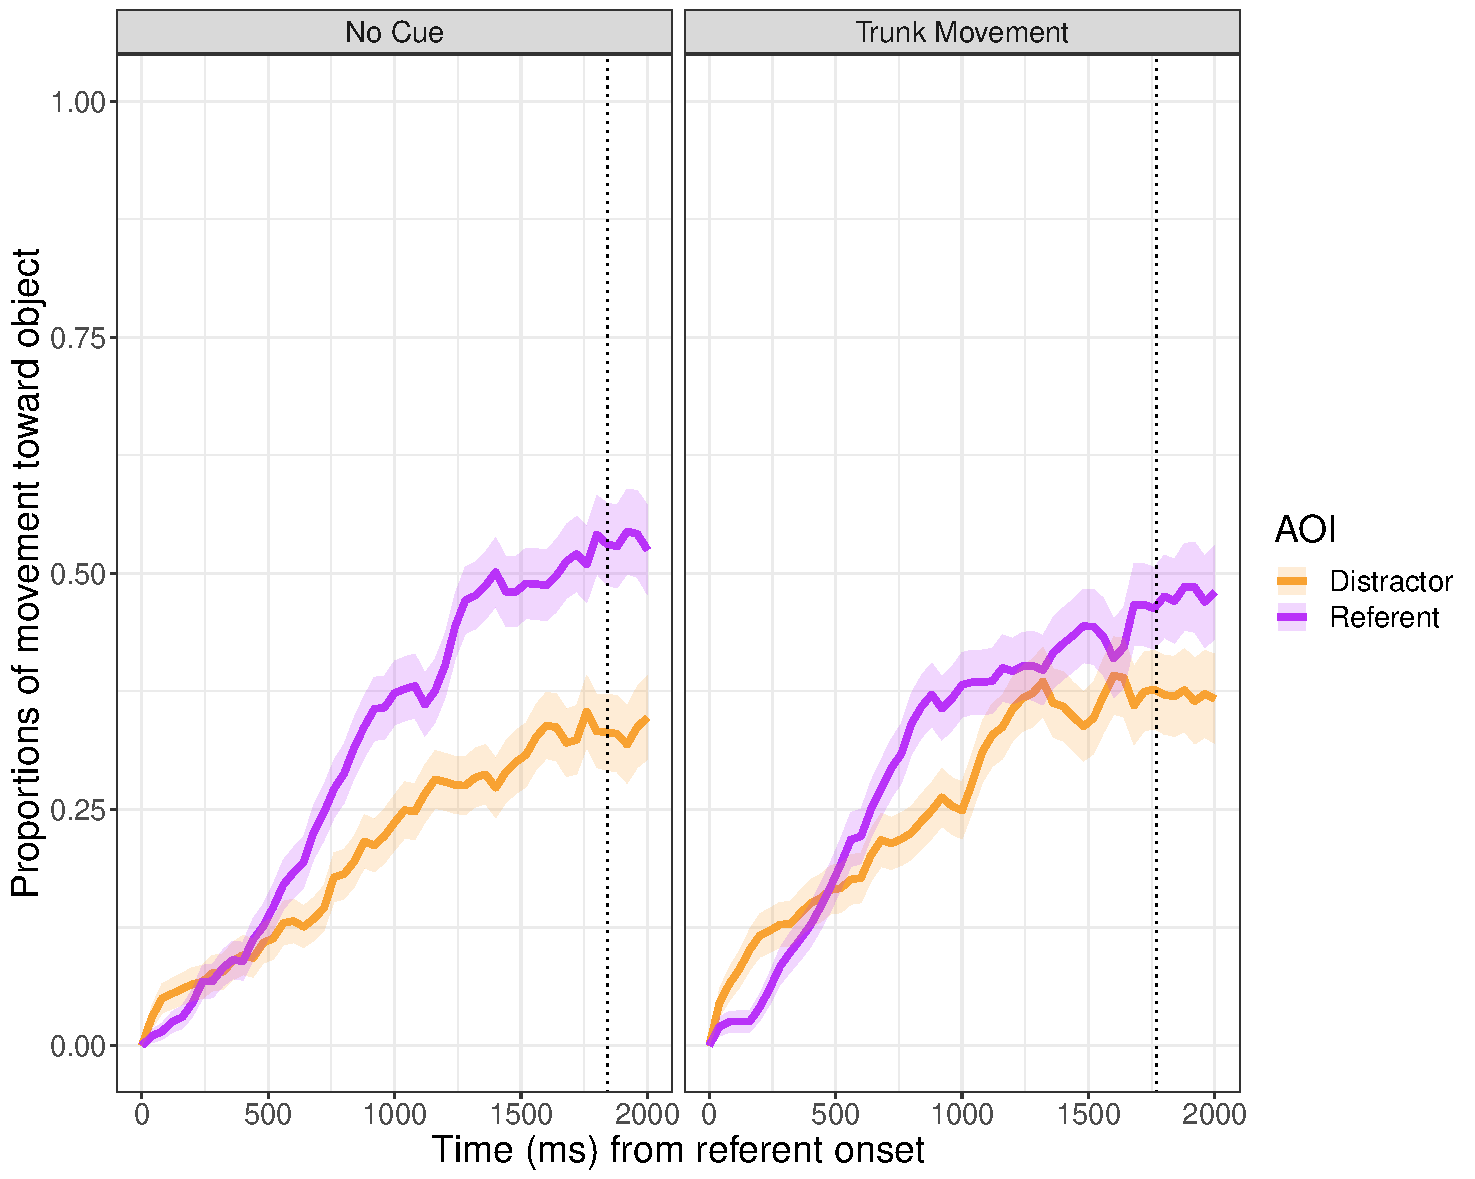
\includegraphics[width=\linewidth]{./img/e7_mouse_crit.pdf}
  \caption{Mouse-tracking results for critical trials in Experiment~1: Proportion of cumulative distance traveled toward each object from 0 to 2000 ms post-referent onset. Proportions were calculated from the total cumulative distance participants moved the mouse until that time bin (from video onset, when cursor was made visible). Shaded areas represent $\pm$ 1 standard error of the mean.}
  \label{fig:v1_mouse1}
\end{figure}

\begin{figure}[Ht]
  \centering
	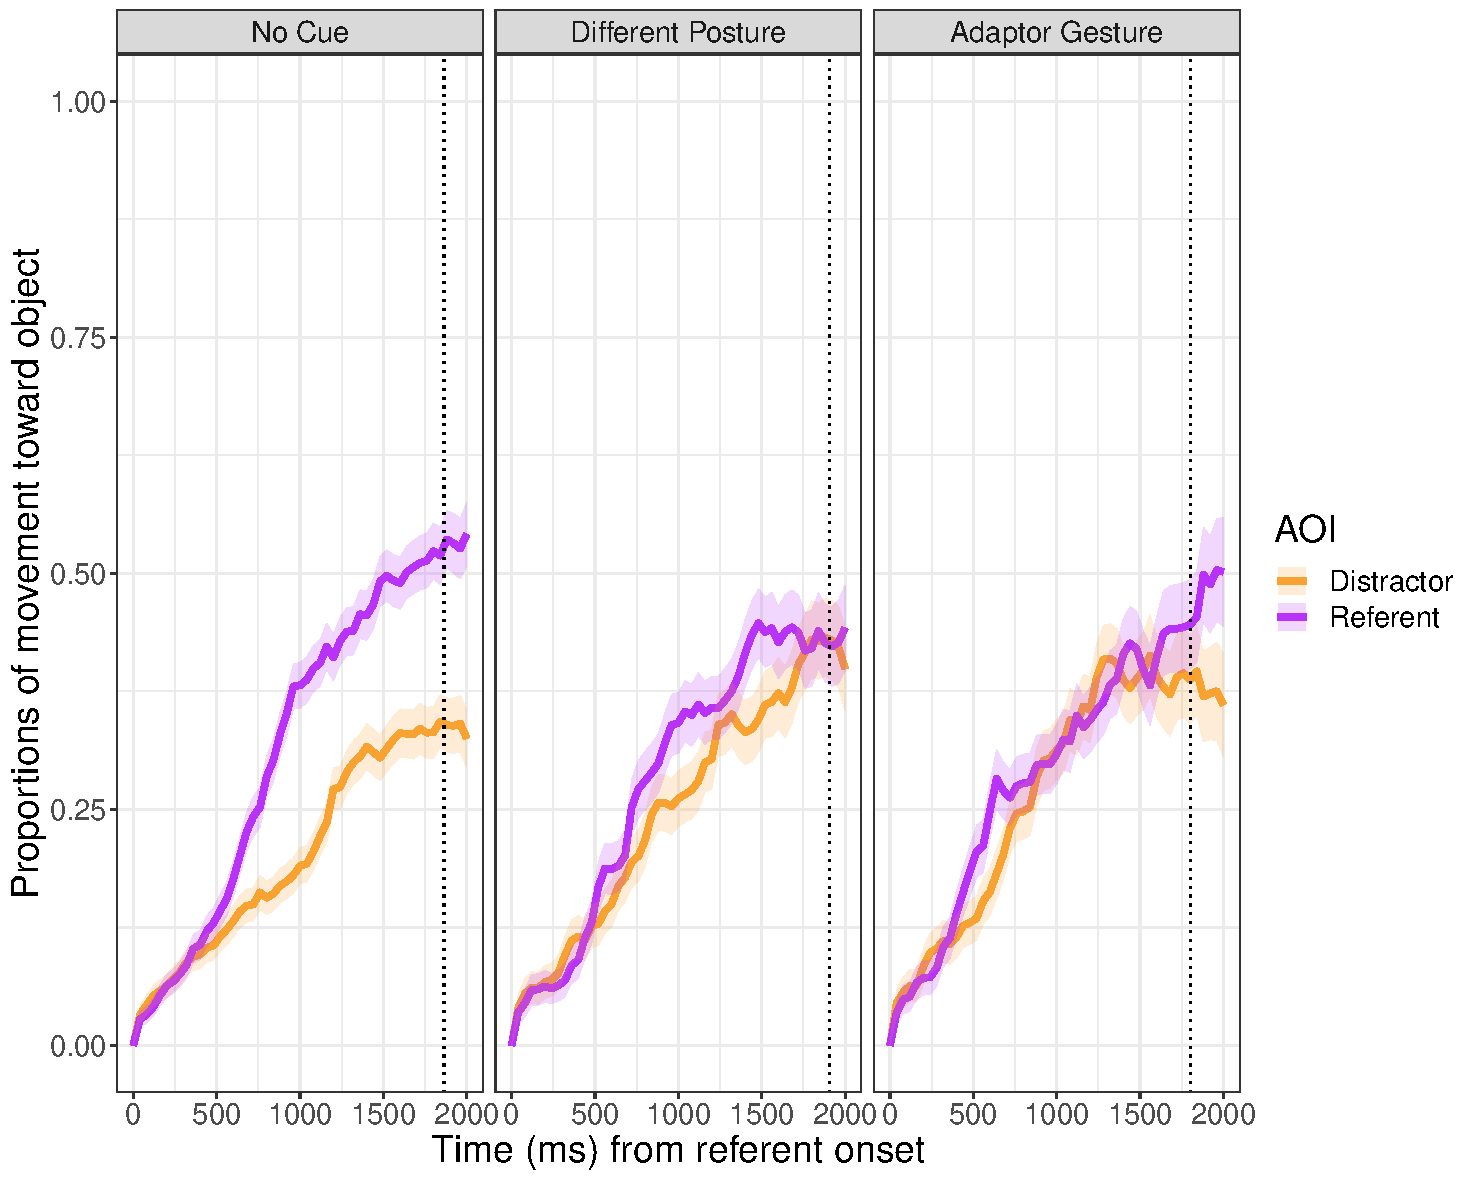
\includegraphics[width=\linewidth]{./img/e7_mouse_filler.pdf}
  \caption{Mouse-tracking results for filler trials in Experiment~1: Proportion of cumulative distance traveled toward each object from 0 to 2000 ms post-referent onset. Proportions were calculated from the total cumulative distance participants moved the mouse until that time bin (from video onset, when cursor was made visible). Shaded areas represent $\pm$ 1 standard error of the mean.}
  \label{fig:v1_mouse2}
\end{figure}


\section{Discussion}
Experiment~1 investigated how the pragmatic inferences listeners make about a speaker's honesty are influenced by the presence of different types of visual cues. 
We measured eye- and mouse- movements of participants who were presented with a task in which they made decisions about the true location of some treasure based on audio and video of a potentially deceptive speaker making a statement about the treasure's location.
Participants were thus making implicit decisions about the honesty of each utterance.
As in previous studies using versions of this paradigm \citep{Loy2017, King2018}, participants showed a tendency to interpret an utterance as truthful when it had been presented without any potential cue to deceit, supporting previous findings in the deception literature that listeners' final judgements of deception are influenced by a speaker's nonverbal behaviour.

Visual information presented alongside utterances was found to influence which object participants clicked on, supporting the previous findings that suggest that a speaker's nonverbal behaviour influences listeners' judgements about (dis)honesty.
However, this claim is only supported by the analysis of filler trials which showed a strong association between the nonverbal behaviour (specifically adaptor gesturing) shown in the videos and participants' final judgements of the utterance as dishonest. 
This effect was marginal in critical trials, which presented videos showing a speaker either producing a trunk movement or sitting motionless.
The influence of the visual channel was also evident in participants' early stages of utterance processing as evidenced in both eye- and mouse- movements, but this effect was again only present in filler trials.
Analysis of both critical and filler trials indicated that when presented with videos of the speaker sitting motionless in a neutral posture, participants showed an initial tendency to fixate and move the mouse toward the referent over the distractor.
This referent-bias was found to be attenuated when videos showed either of the cues (different postures or adaptor gesturing) included in filler trials.

Results from Experiment~1 suggest that adaptor gesturing may be more strongly associated with deception than trunk movements, as evidenced by their influence on the final judgements participants made about utterance veracity.
This contrasts with our prediction that trunk movements would provide the best opportunity to investigate the association between visual cues and deception-judgements.
One possible explanation for this could be due to the fact that at the point of referent onset, the audiovisual information immediately available to the listener was comparable to the no-cue videos (the trunk movements having ended at speech onset).
For videos showing other types of visual cue, the cues either stopped closer to referent onset (adaptor gestures) or were ongoing (different postures).
Despite the fact that these videos showed movement in a smaller area of the video (or no movement at all), their proximity in time to critical noun may explain the difference found relative to trunk movements.
This explanation, however, is at odds with the bias towards judgements of deception following utterance-initial disfluencies observed in previous work \citetext{\citet{Loy2017}, Experiment~1}.
We cannot at present reconcile this discrepancy, although we suggest that they may point toward differences in the mechanisms underlying the integration of audio and visual cues with a pragmatic inference.
Future research could explore the simultaneous integration of audio and visual information during judgements of deception, comparing the relative time course with which the two are integrated by the comprehension system.

From a practical viewpoint, these findings suggest that use of the visual world paradigm to investigate linguistic processing is compatible with the inclusion of a video stimulus.
Our choice to focus on trunk movements was in part motivated by their visual saliency and temporal coordination with speech (appearing prior to, and not alongside, speech), but this may have been unnecessarily cautious: 
Videos showing adaptor gesturing simultaneously with utterance playback did not detract from a fixation bias appearing in the early stages of reference comprehension, and small movements such as finger tappings were salient enough to influence judgements of deception.
Trunk movements, however, were the only type of visual cue which was fully counterbalanced in our design.
Videos including adaptor gestures or different postures were not counterbalanced across referents, nor were the frames at which audio began playing matched by videos showing no cue (although this difference is extremely minimal--- on average 1 frame, or 40~ms).
Additionally, 25\% of the filler trials were presented as ``hidden bonus rounds'', providing participants with explicit feedback on their judgement, and potentially influencing our findings. 

Aiming to clarify the time course of visual cue based judgements of deception, we conducted Experiment~2, in which there was no feedback given, and participants saw videos in only two different conditions: showing an adaptor gesture, or showing no cue. 
Additionally, in the verbal questioning after the experiment, several participants mentioned basing their judgements on \spex{how relaxed the speaker looked}, and adaptor gestures have been suggested to be characteristic of body-language associated with anxiety \citep[see][]{Gregersen2005}.

\section{Experiment~2}
Using the same paradigm as Experiment~1, participants in Experiment~2 heard utterances accompanied by a video of a speaker either producing an adaptor gesture or sitting motionless, and were tasked with making an implicit judgement on whether the speaker was lying or telling the truth.
In the post-test questions after Experiment~1, several participants mentioned basing their judgements on \spex{how relaxed the speaker looked}, so in Experiment~2 we used a selection of adaptor gestures which are associated with nervousness based on \citet{Gregersen2005}, which were pre-tested for perceived anxiety in the speaker.
As a manipulation check, after the treasure-game task, participants were asked to rate each video (without audio) on how nervous the speaker looked.

\subsection{Materials}
The 40 images used in critical trials in Experiment~1 (20 referents; 20 distractors) were used across twenty trials.
As in Experiment~1, these images were displayed in referent-distractor pairs, with each pair shown alongside a recorded utterance naming the referent as the location of the treasure.
Following \citet{Loy2017}, these were the referents and distractors which had been matched for both ease of naming and familiarity.
The pairing of referents and distractors on each trial was randomised.

As in Experiment~1, each pair of images and recorded utterance was presented alongside a video clip of a person purported to be the speaker of the utterance.
Twenty-eight new video clips were recorded (18 different adaptor gestures; 10 no-cue). 
Care was taken to ensure that the videos including no cue showed the speaker in a relaxed posture. 
Adaptor gestures were based on descriptions of anxious nonverbal behaviour from \citet{Gregersen2005}.
All 28 videos were pre-tested for perceived nervousness of the speaker.
Ten native english speakers were told that they were going to watch videos (without audio) of someone being questioned in a stressful situation, and were asked to rate how nervous the speaker looked in each video (1: very relaxed, 7: very nervous). 
The 10 videos showing adaptor gestures with the highest ratings (Mean = 4.1, SD = 1.5) were included in the experiment, along with the 10 videos showing no cue (Mean = 1.9, SD = 1.1).

The 20 referents were counterbalanced across two lists such that each referent that occurred with a video showing adaptor gesturing in the first list occurred with a video showing no cue in the second.
The pairings of referents with specific videos within each condition was randomised on each run of the experiment.

\subsection{Procedure}
The experiment procedure was identical to that of Experiment~1 with the following changes.
First, the size of the video stimuli changed slightly, and measured 236~$\times$~336 pixels.
Second, the number of video frames presented prior to the audio recording beginnig was set at a fixed constant of 35 (equating to 1400~ms).
Third, we did not include any `bonus' trials which displayed a message stating that treasure had been found after an object click, meaning participants did not receive any feedback throughout the experiment.

After the main task, participants were asked to watch all 20 videos again, without audio, and asked to rate how nervous they thought the speaker looked (using the same 1-7 scale as described above).
Participants then completed the same post-test questionnaire as in Experiment~1, with data being excluded from analysis based on the same criteria.

\section{Results}
Twenty-three native English speaking participants took part in exchange for \pounds{}3 compensation for a desired sample size of twenty. 
Data from three participants were excluded due to suspicion of the audiovisual stimuli being scripted (based on the post-test questionnaire and questioning during debrief), hence the final dataset included data from 20 participants.

\subsection{Analysis}
We followed the same analysis strategy as was used for Experiment~1, with the experimental manipulation now no cue vs.\@ adaptor gesture.
Trials which did not result in a click to either object (3) were excluded from analyses, leaving 397 trials.
Mouse-movements beyond the outer edge of either object were excluded from analyses (1\% of samples)
Analyses was identical to that of the critical trials in Experiment~1

\subsection{Object clicks}
Across the experiment, participants clicked on the referent in 53\% of trials and the distractor in 47\%.
Table \ref{table:v2_clicks} shows the proportions of clicks to either object following videos showing different types of cue (no cue vs.\@ adaptor gestures).
As in Experiment~1, participants showed a bias toward a final interpretation of the utterances accompanied by videos with no cue as truthful, with more clicks to the referent than the distractor \resultsLog{1.39}{0.19}{<0.001}.

The time participants took to click on an object was not influenced by whether the video showed an adaptor gesture or no cue.

\begin{table}
\caption{Breakdown of mouse clicks recorded on each object (referent or distractor) by cue type for Experiment~2}
\label{table:v2_clicks}
\begin{tabularx}{\linewidth}{YYY}
\hline
& No Cue & Adaptor gesture \\
Clicks to Referent & 161 (80.9\%) & 48 (24.2\%)  \\
Clicks to Distractor & 38 (19.1\%) & 150 (75.8\%)  \\
\hline
\end{tabularx}
\end{table}


\subsection{Eye movements}
Figure \ref{fig:v2_eye} shows the time course of fixations to referents and distractors over 2000~ms from referent onset, split by whether the video showed no cue or adaptor gesturing.
Analyses conducted over the period from referent onset to 800~ms post-onset patterned with participants responses to adaptor gesturing in Experiment~1: 
When presented with an utterance unaccompanied by a video showing no cue, participants displayed a fixation bias towards the referent which increased over time (\resultsLM{2.99}{0.67}{=4.48}).
When presented with an utterance accompanied by video of an adaptor gesture, this bias was greatly reduced (\resultsLM{-2.94}{0.20}{=-14.27}).

\begin{figure}[Ht]
  \centering
	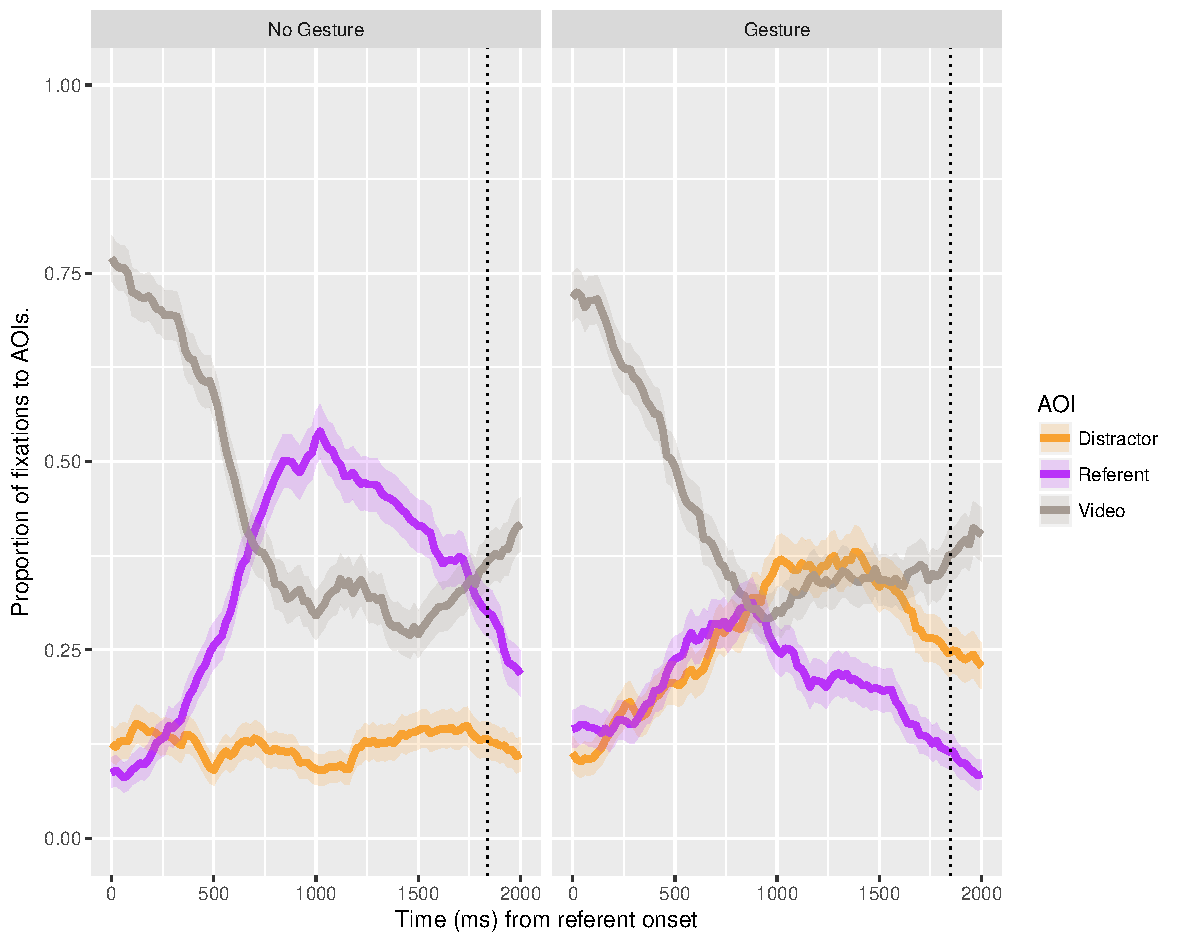
\includegraphics[width=\linewidth]{./img/e8_fixations.pdf}
  \caption{Eye-tracking results for Experiment~2: Proportion of fixations to each object (referent or distractor) and the video, from 0 to 2000 ms post-referent onset, calculated out of the total sum of fixations for each 20~ms time bin. Shaded areas represent $\pm$ 1 standard error of the mean.}
  \label{fig:v2_eye}
\end{figure}

\subsection{Mouse movements}
Figure \ref{fig:v2_mouse} shows the time course of the proportions of cumulative distance the mouse moved towards the referent and distractor for 2000~ms from referent onset, split by cue type.
Mouse-movements over the course of the 800~ms window from referent onset again patterned with the eye-tracking data:
Following videos showing no cue, participants showed a tendency to move the mouse increasingly towards referent over this period (\resultsLM{1.77}{0.31}{=5.72}), but this increasing referent-bias was greatly reduced following videos showing an adaptor gesture (\resultsLM{-2.16}{0.19}{=-11.40})

\begin{figure}[Ht]gesture
  \centering
	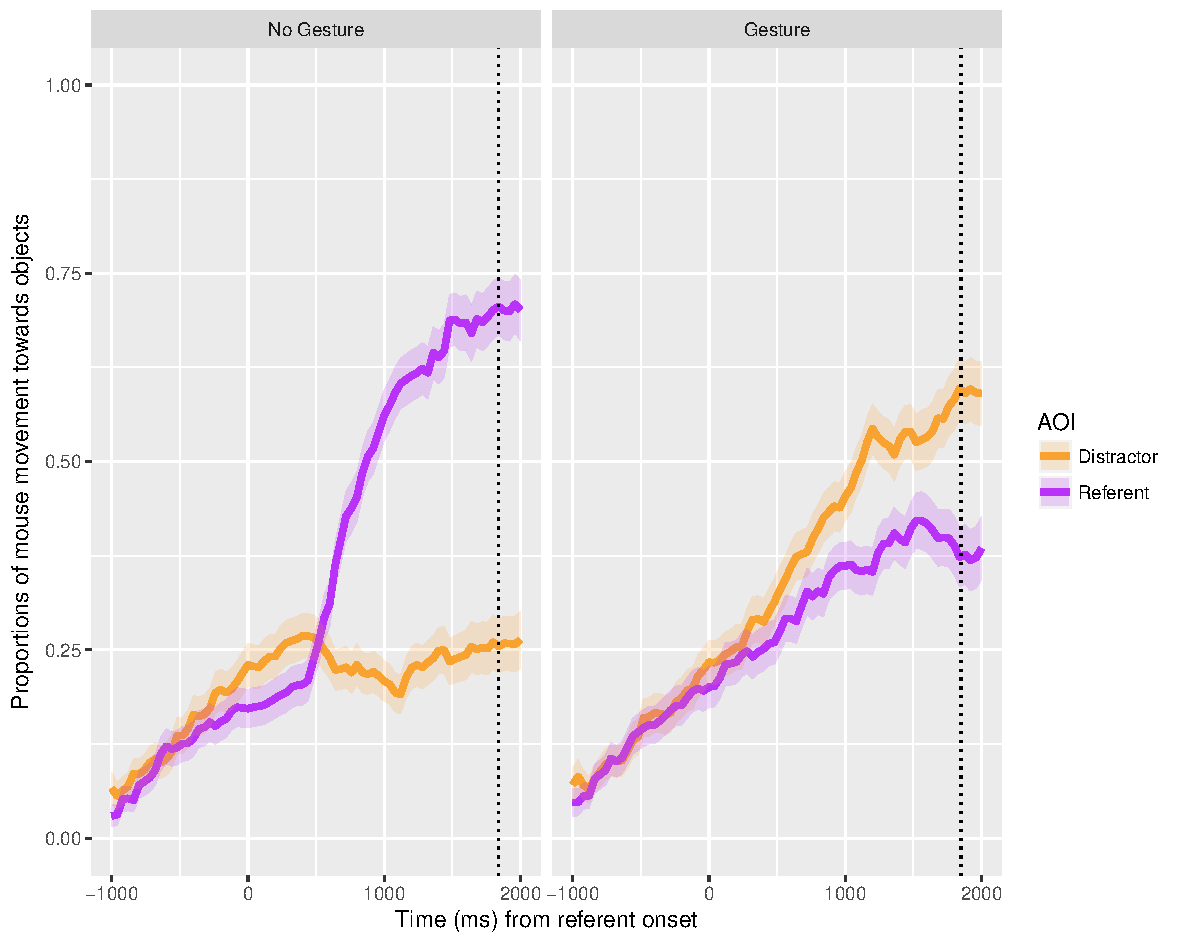
\includegraphics[width=\linewidth]{./img/e8_mouset.pdf}
  \caption{Mouse-tracking results for Experiment~2: Proportion of cumulative distance traveled toward each object from 0 to 2000 ms post-referent onset. Proportions were calculated from the total cumulative distance participants moved the mouse until that time bin (from speech-onset, when cursor was made visible). Shaded areas represent $\pm$ 1 standard error of the mean.}
  \label{fig:v2_mouse}
\end{figure}


\section{General discussion}
The studies presented here investigate the integration of visual information about a speaker into judgements of deception.
We manipulated the presentation of the different non-verbal behaviours while measuring eye- and mouse- movements of the listener towards one of two possible final judgements about the veracity of an utterance.
In doing so, we explored the possibilities of whether listeners are relying upon a rule-of-thumb heuristic in associating visual cues to deception, or whether the link between nonverbal behaviour and perceived deception requires a more complex inferential process.

In Experiment~1, listeners' final interpretations of utterance veracity were influenced by visual information about the speaker which was presented concurrently with presentation of speech.
However, these findings were only apparent in relation to visual cues used in filler trials (in which videos showed a speaker in different postures and producing adaptor gestures), with a marginal effect of the trunk movements which were the focus of the study.
Analysis of the filler trials in Experiment~1 indicated that visual information about a speaker can be integrated into the early stages of reference comprehension, and that this information can be both static and dynamic.
Experiment~1 also showed that the visual world paradigm can be adapted to include video stimuli of the speaker without detracting from fixation-biases, even when this video stimuli is changing during the presentation of speech.
This aligns with research suggesting that listeners may extract information about gestures through peripheral vision \citep[See e.g.][]{Gullberg2006}.
To directly investigate the time-course of judgements based on adaptor gestures in a fully counterbalanced design, we conducted Experiment~2, which confirmed that participants engaged in rapid integration of visual information into pragmatic judgements of deception.

The findings presented here are consistent with previous research on beliefs about and judgements on visual cues to deception showing that listeners perceive a range of nonverbal behaviours to indicate deceit \citep[e.g.][]{Zuckerman1981, Akehurst1996, Vrij2000}, and provides a visual-modality parallel with the findings from \citet{Loy2017} showing that fluency of speech influences judgements of whether a speaker is lying
Our findings, together with those from \citet{Loy2017}, suggest that listeners may have an implicit bias to judge a speaker as honest in the absence of any obvious potential cue to deception. 
Additionally, they align with the `truth bias' commonly observed in deception literature, in which listeners have a tendency to judge a speaker as truthful, even when explicitly told the speaker may be dishonest \citep{Vrij2000}.

The time course of listeners' eye- and mouse-movements showed that the influence of the visual channel is apparent during the early stages of comprehension:
In both experiments, utterances presented with the speaker in a neutral posture and not gesturing biased listeners towards believing the speaker to be truthful, as shown by increased tendency to fixate on, move the mouse towards, and eventually click on the object which was named by the speaker. 
In contrast, utterances presented alongside a visual cue such as an adaptor gesture significantly reduced this bias, as evidenced in Experiment~2.
Importantly, this difference emerged during the initial stages of linguistic processing, with effects found in Experiment~2 during the same time-window as that in which \citet{Loy2017} found effects of speech disfluency.
Just like manner of spoken delivery, the manner of visual delivery can very quickly modulate a listeners' judgements about the speaker's intentions alongside processing of the lexical information. 

Although it is tempting to interpret these results as indicative of participants relying on heuristically associating visual cues with lying, visual inspection of the time course suggests that this might not be the case.
When presented with a video showing a speaker producing an adaptor gesture, the bias towards the distractor --- signifying perceived dishonesty --- over the referent appeared approximately 1000~ms after the referent began, at a later point than previous versions of this paradigm in which speech disfluencies were found to modulate judgements of deception. 
This time course of events is difficult to reconcile with a view that listeners are relying on rule-of-thumb associations between visual cues and deception, and could suggest that listeners may be engaging in a more complex reasoning process in integrating manner of visual delivery than manner of spoken delivery. 

Our results show that the integration of the visual channel in utterance processing can have a rapid and direct effect on a listener's pragmatic judgements, supporting the idea that communication is fundamentally multimodal: 
Speech and gesture interactively codetermine meaning.
However, the integration of visual cues to inform deception judgements appears to be more gradual than the integration of spoken cues.
To better understand how information in different modalities affect comprehension, further research would require investigating the effect of spoken delivery when the visual channel is also available --- for example, studying the time course of deception judgements when faced with one or both of a disfluency and an adaptor gesture.


\bibliography{./GCD}

\end{document}
